% =====================================================
% SLIDE: DATASET & FEATURE ENGINEERING
% =====================================================
\section{Dataset \& ML}
\begin{frame}{2. Dataset \& Feature Engineering}
    \framesubtitle{Rubric: Methodology -- Datasets \& Preprocessing}
    \small
    \begin{itemize}
        \item \textbf{Published Benchmark Dataset (Kaggle):} Open-sourced on \href{https://www.kaggle.com/datasets/mouniksai/vehicular-misbehavior-dataset-edgetrust-vanet/data}{\textbf{\underline{Kaggle}}} (\texttt{EdgeTrust-VANET}) for community reproducibility.
        
        \item \textbf{Multi-Source ETL Harmonization (23{,}970 records):} Standardized 3 corpora into a unified schema: \textbf{VeReMi (72.9\%)}, \textbf{EdgeTrust-VANET (20.9\%)}, \textbf{V-RADD (6.3\%)} [70.6\% Benign, 29.4\% Attack across 6 vectors].
        
        \item \textbf{14 RSU-Observable Features Derived (Zero Leakage):}
        \begin{itemize}
            \item \textbf{Mobility (5):} Coordinates ($x, y$), speed, heading, acceleration.
            \item \textbf{Network (6):} Packets sent/received, drop ratio, latency, retransmissions, RSSI.
            \item \textbf{Trust Engine (3):} Direct trust ($T_t$), 300\,m KD-Tree neighbor avg, historical trust.
        \end{itemize}
        
        \item \textbf{Zero-Leakage Group Splitting:} Purged 4 post-hoc label counters ($100\% \to 86.05\%$ without them); partitioned strictly by \textbf{Vehicle ID (\texttt{node\_id})} (70/15/15) to eliminate trajectory autocorrelation.
        
        \item \textbf{Rigorous 2-Stage Evaluation:}
        \begin{itemize}
            \item \textbf{Validation (Split Dataset):} \textbf{97.74\% F1} / \textbf{97.77\% Acc} (5-fold CV: \textbf{96.95\% $\pm$ 1.12\%}).
            \item \textbf{Testing (Live OMNeT++/Veins RSU):} \textbf{90.99\% Acc} / \textbf{90.97\% F1} on 2{,}331 packets.
        \end{itemize}
    \end{itemize}
\end{frame}

% =====================================================
% SLIDE: ML MODEL TRAINING & BENCHMARK RESULTS
% =====================================================
\begin{frame}{3. Model Validation \& Live RSU Testing Benchmark}
    \framesubtitle{Rubric: Core Algorithms \& Evaluation Metrics}
    \begin{columns}
        \column{0.48\textwidth}
        \scriptsize
        \begin{itemize}
            \item \textbf{17 Models Evaluated} across Ensembles, GBDTs, Linear, Kernel, and Neural Network architectures.
            
            \item \textbf{Validation (Split Dataset -- 3{,}539 samples):}
            \begin{itemize}
                \item 5-Fold Stratified Group CV: \textbf{96.95\% $\pm$ 1.12\%}.
                \item Top models: RF (\textbf{97.77\% Acc}, \textbf{97.74\% F1}), LightGBM (\textbf{97.74\% Acc}), CatBoost (\textbf{97.29\% Acc}).
            \end{itemize}
            
            \item \textbf{Testing (Live OMNeT++/Veins RSU -- 2{,}331 pkts):}
            \begin{itemize}
                \item \textbf{\#1 Top Champion:} \textbf{Random Forest} -- \textbf{90.99\% Test Acc}, \textbf{90.97\% Test F1}, lowest missed attack rate (\textbf{6.89\%}).
                \item \textbf{Ultra-Fast Edge Leaders:} \textbf{LogReg \& LDA} -- \textbf{89.28\% Test F1}, \textbf{82.8 $\mu$s} latency ($>12{,}000$ pkt/s), \textbf{1.0 KB} footprint.
                \item \textbf{Top Edge GBDT:} \textbf{CatBoost} -- \textbf{79.79\% Test F1}, \textbf{90.77\% ROC-AUC}, \textbf{118.3 $\mu$s}, 248 KB.
            \end{itemize}
            
            \item \textbf{Key Live Finding:} Live radio jitter caused MLP/SVM to collapse (FAR $>97\%$), while Tree Ensembles remained robust.
        \end{itemize}
        \column{0.52\textwidth}
        \centering
        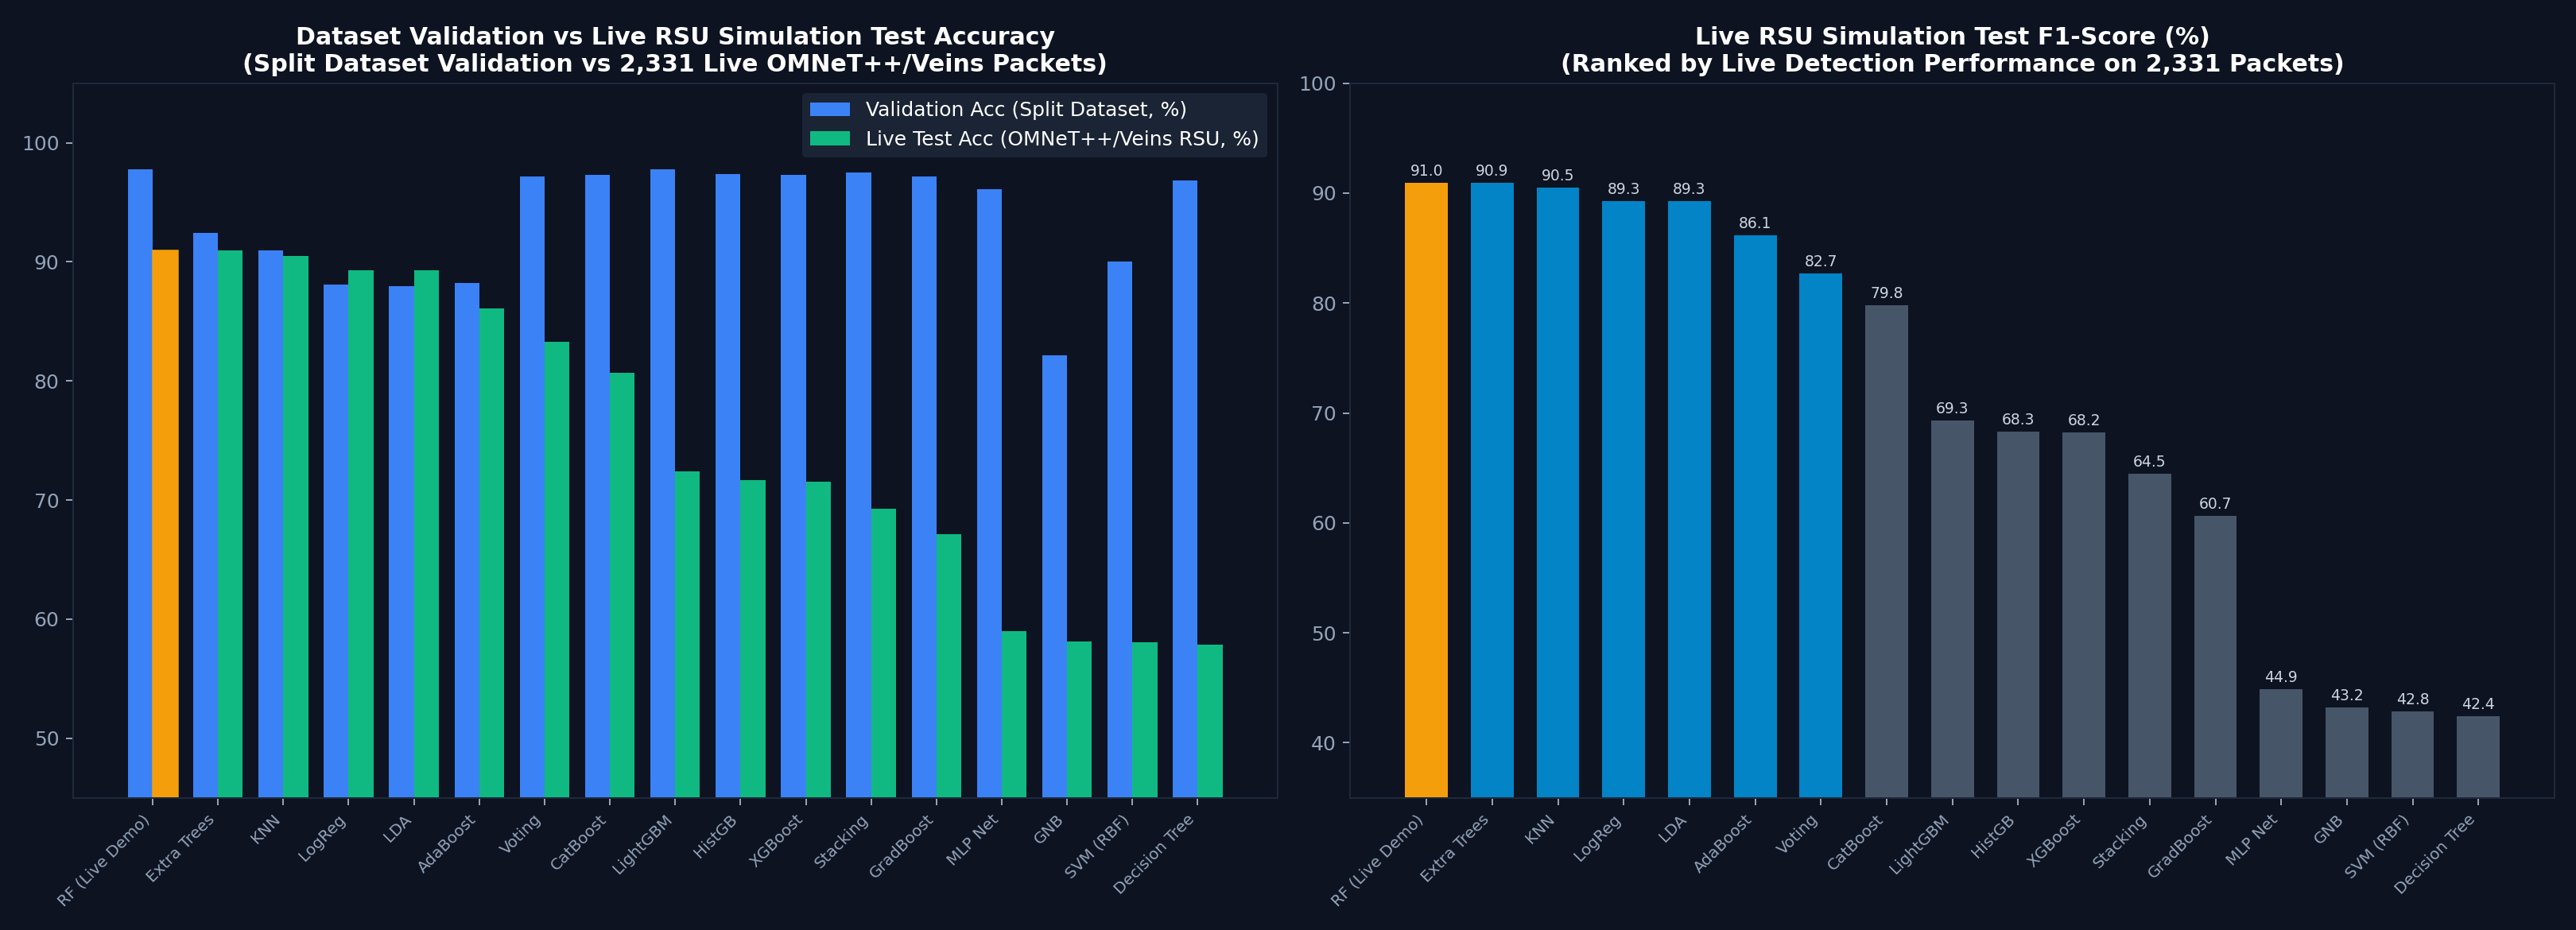
\includegraphics[width=\linewidth,keepaspectratio]{vanet_comparison.png}
    \end{columns}
\end{frame}

% =====================================================
% SLIDE: FEATURE IMPORTANCE & TRUST FORMULA
% =====================================================
\begin{frame}{4. Feature Importance \& Edge Trust Score Formula}
    \framesubtitle{Rubric: Mathematical Model / Formulation}
    \begin{columns}
        \column{0.55\textwidth}
        \centering
        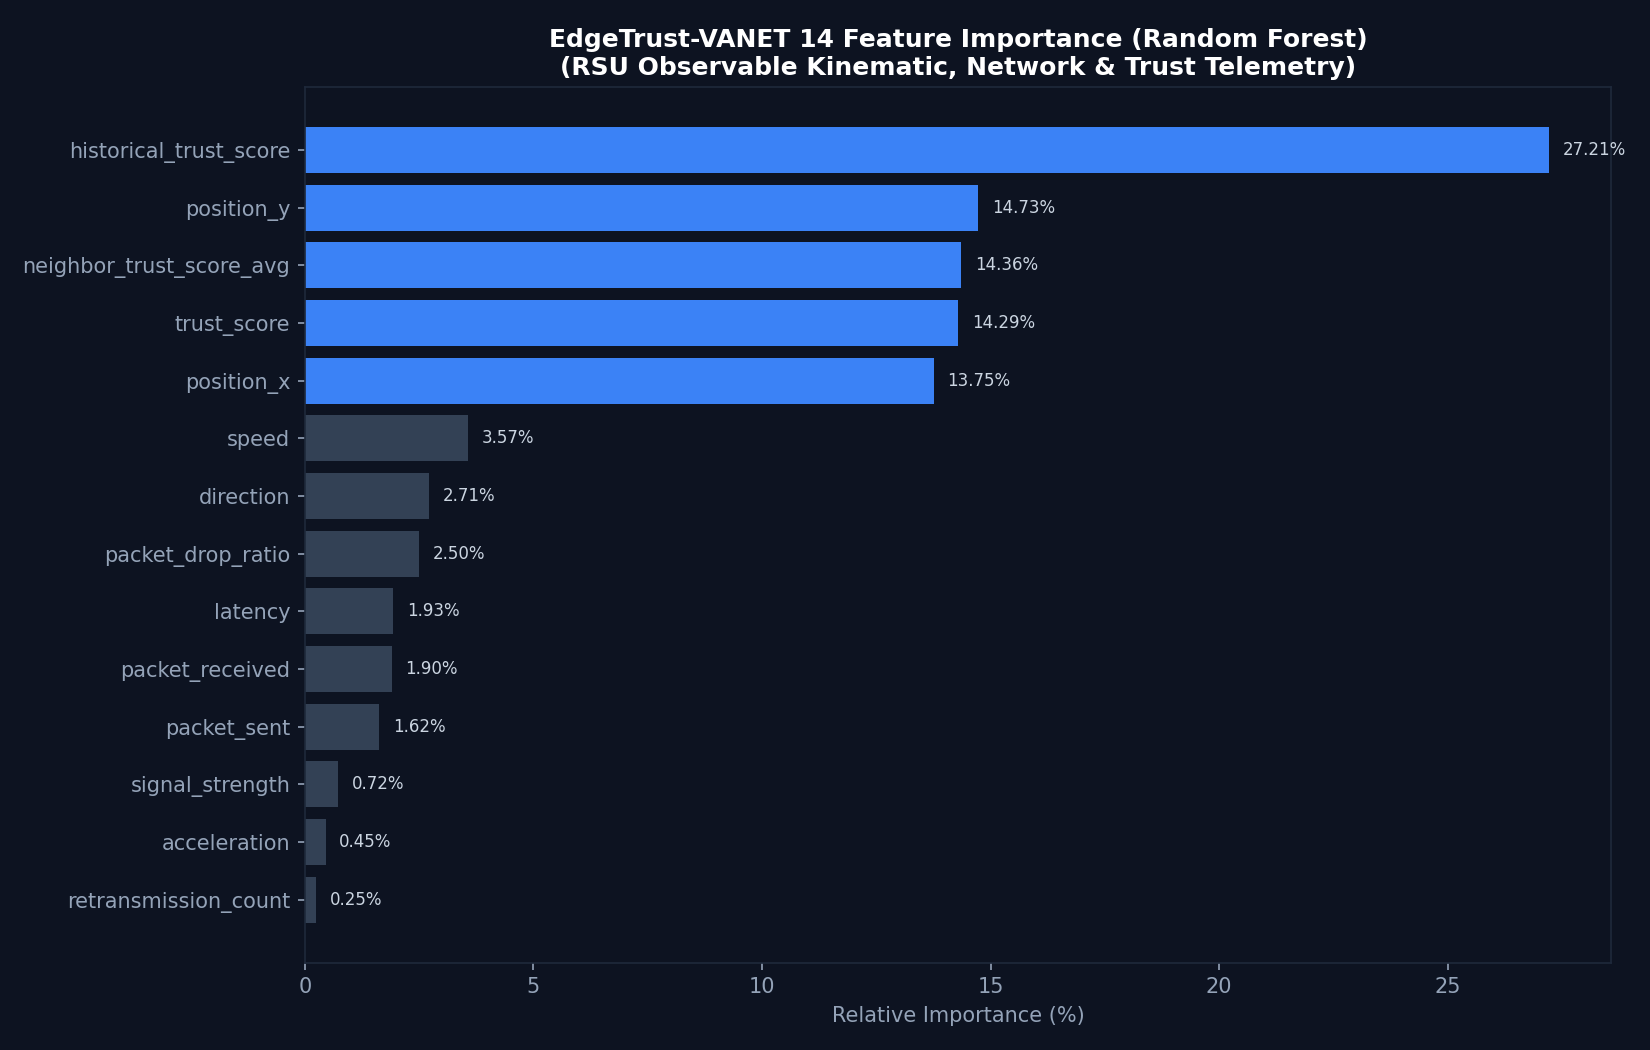
\includegraphics[width=\linewidth,height=0.78\textheight,keepaspectratio]{vanet_feature_importance.png}
        \column{0.45\textwidth}
        \footnotesize
        \begin{itemize}
            \item \textbf{Trust features dominate (55.86\%):} \texttt{historical\_trust\_score} (27.21\%), \texttt{neighbor\_trust\_score\_avg} (14.36\%), and \texttt{trust\_score} (14.29\%) explain more than half of all model decisions.
            \item \textbf{Kinematic \& network signals (44.14\%):} Spatial consistency ($p_x, p_y$: 28.48\%), speed (3.57\%), heading (2.71\%), packet drop ratio (2.50\%), and latency (1.93\%).
        \end{itemize}
        \vspace{0.2cm}
        \textbf{Heuristic Trust Update (EMA):}
        \[
        T_t = \alpha \cdot T_{t-1} + (1-\alpha)\cdot E_t
        \]
        {\scriptsize $T_t$: current trust, $T_{t-1}$: historical trust, \\ $\alpha = 0.70$ (memory retention factor), \\ $E_t \in [0, 1]$: observable real-time evidence:
        \[
        E_t = 0.35 E_{\text{mobility}} + 0.30 E_{\text{delivery}} + 0.20 E_{\text{latency}} + 0.15 E_{\text{channel}}
        \]
        Spatial neighbor trust computed via 300m KD-Tree.}
    \end{columns}
\end{frame}

% =====================================================
% ADDITIONAL SLIDE: ALPHA TRUST UPDATE ANALYSIS
% =====================================================
\begin{frame}{Why $\alpha = 0.70$ in the Hybrid Trust Update}
    \framesubtitle{Rubric: Sensitivity Analysis \& Parameter Justification}
    \begin{columns}
        \column{0.62\textwidth}
        \centering
        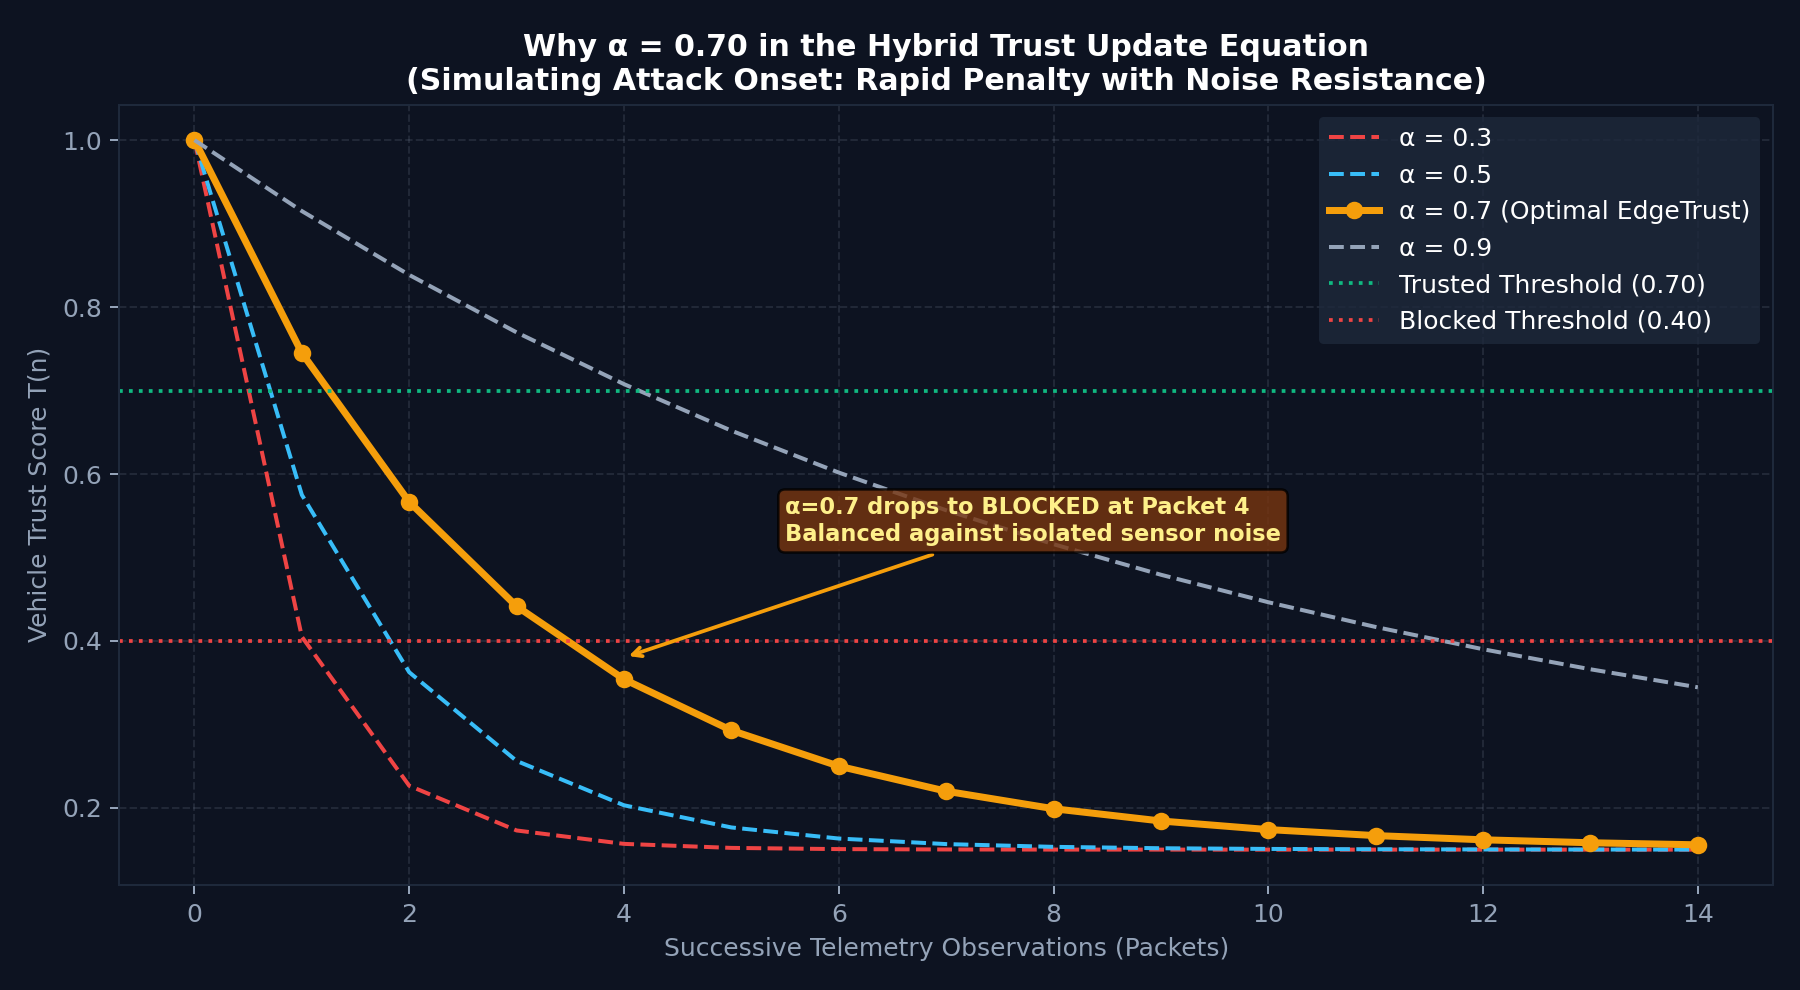
\includegraphics[width=\linewidth,keepaspectratio]{alpha_trust_update.png}
        \column{0.38\textwidth}
        \footnotesize
        \begin{itemize}
            \item \textbf{Sensitivity Trade-off:}
            \begin{itemize}
                \item $\alpha = 0.3$: Too responsive; transient channel fading/noise causes false punishment.
                \item $\alpha = 0.9$: Too sluggish; requires $>15$ malicious packets before flagging.
                \item $\mathbf{\alpha = 0.70}$ \textbf{(Optimal):} Swiftly degrades malicious trust below the \textbf{0.40 Blocked threshold by Packet 4}, while absorbing isolated benign telemetry noise.
            \end{itemize}
            \item Prevents sudden false disconnects for honest ambulances and braking vehicles.
        \end{itemize}
    \end{columns}
\end{frame}

% =====================================================
% ADDITIONAL SLIDE: EDGE RSU TRADE-OFF ANALYSIS
% =====================================================
\begin{frame}{Edge RSU Deployment: Accuracy vs. Speed \& Footprint}
    \framesubtitle{Rubric: Hardware Feasibility \& Microcontroller Deployment}
    \begin{columns}
        \column{0.62\textwidth}
        \centering
        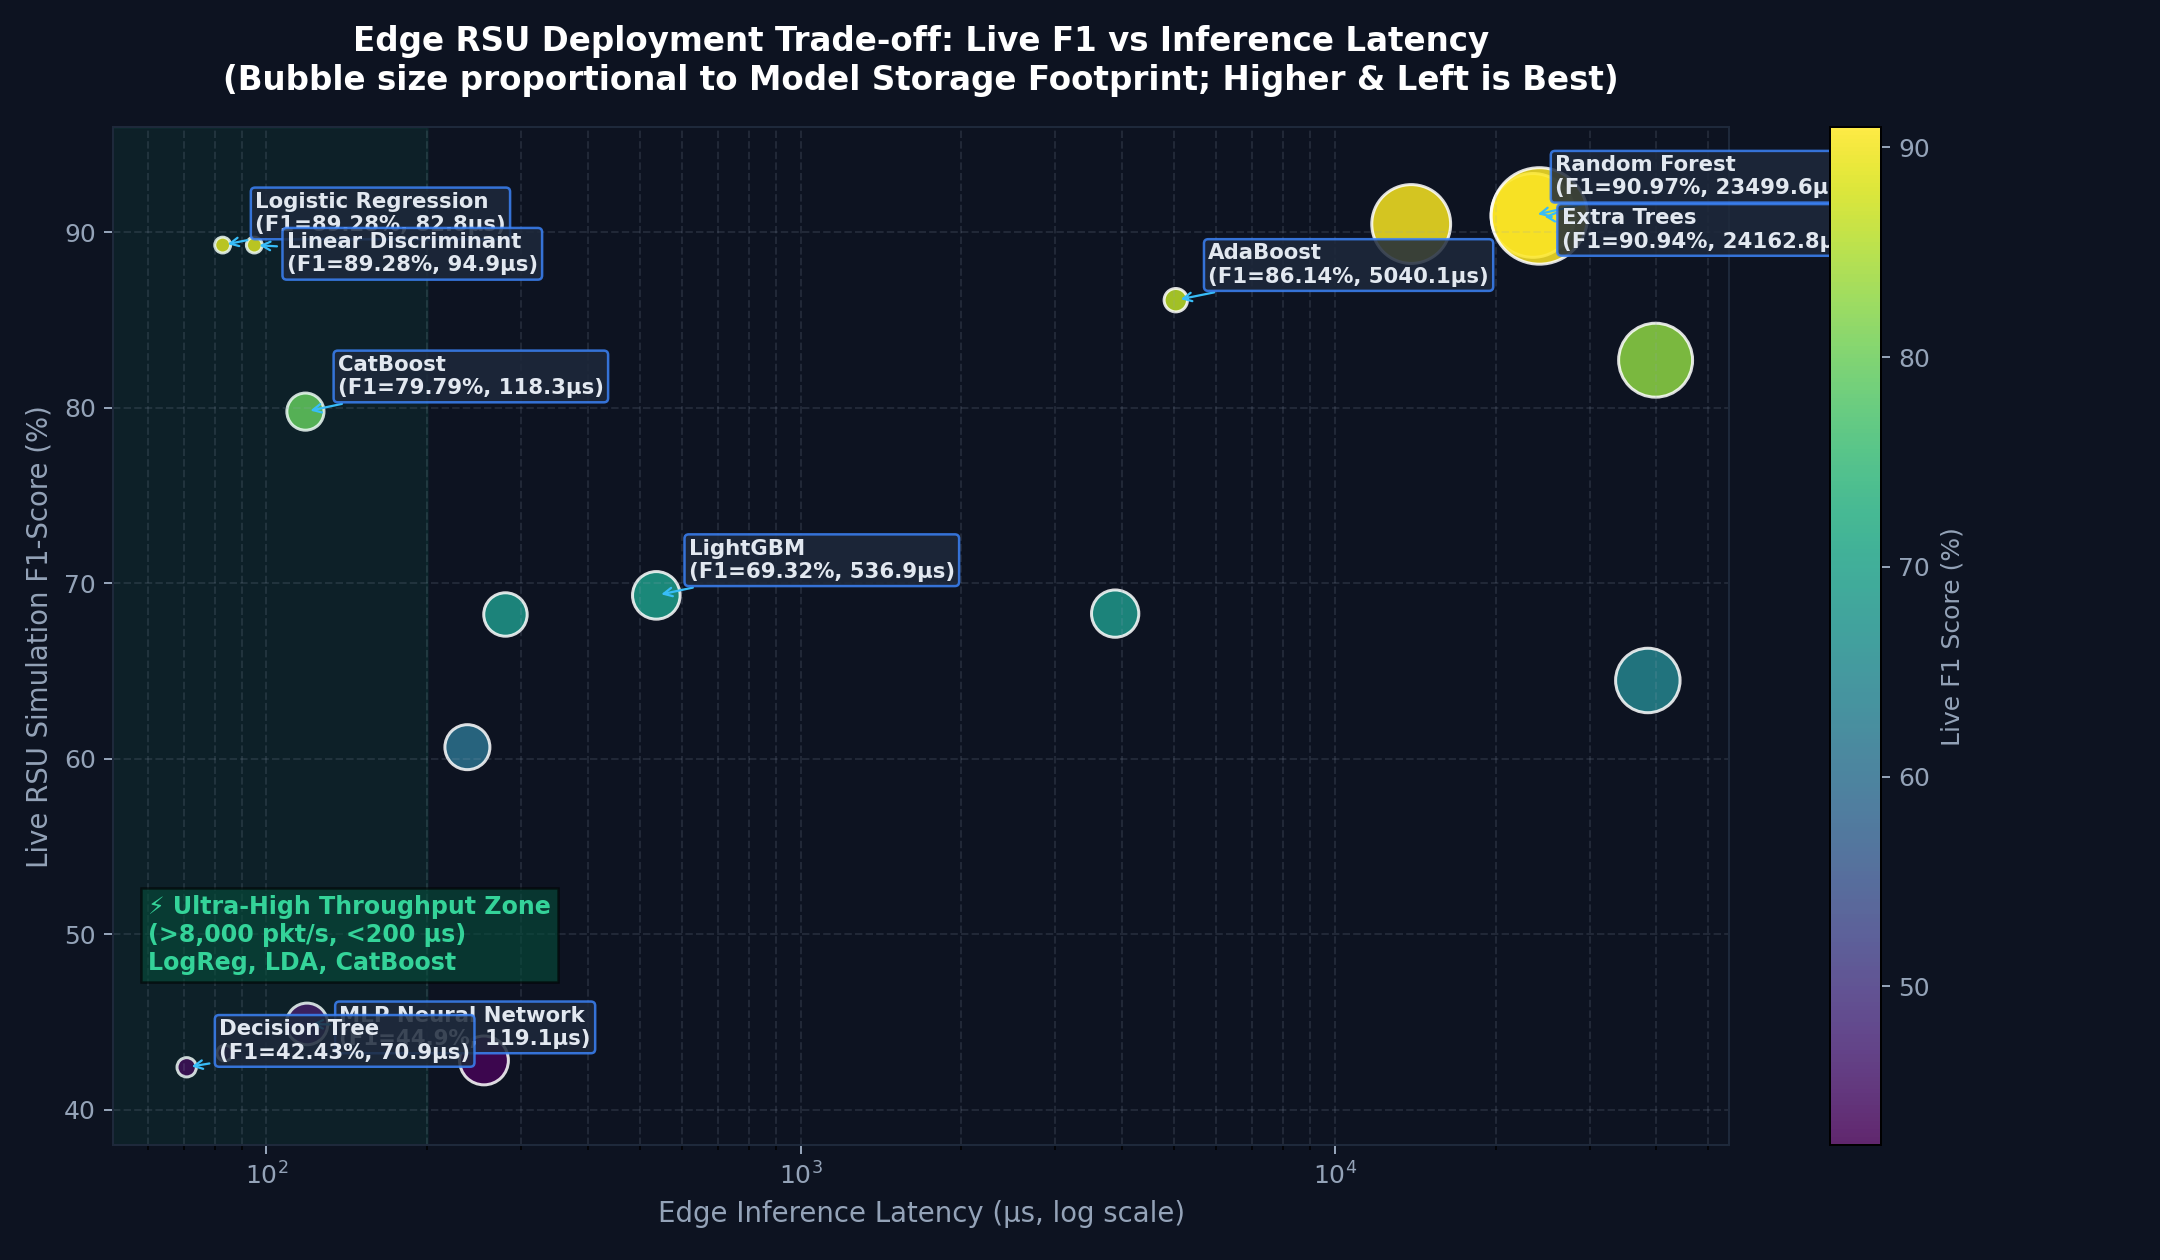
\includegraphics[width=\linewidth,keepaspectratio]{edge_rsu_tradeoff.png}
        \column{0.38\textwidth}
        \footnotesize
        \begin{itemize}
            \item \textbf{RSU Hardware Trade-off:}
            \begin{itemize}
                \item \textbf{Multi-Core Edge Servers:} \textbf{Random Forest} yields top performance (\textbf{97.77\% Val Acc}, \textbf{90.99\% Live Test Acc}, \textbf{90.97\% Live F1}) and lowest missed attacks (\textbf{6.89\%}).
                \item \textbf{Ultra-Constrained RSUs:} \textbf{Logistic Regression \& LDA} execute in \textbf{82.8 $\mu$s} ($>12{,}000$ pkt/s) with a tiny \textbf{1.0 KB} footprint and \textbf{89.28\% Live Test F1}.
                \item \textbf{Balanced GBDT:} \textbf{CatBoost} delivers \textbf{8{,}452 pkt/s} at \textbf{118 $\mu$s} latency and \textbf{248 KB} footprint with 90.77\% ROC-AUC.
            \end{itemize}
        \end{itemize}
    \end{columns}
\end{frame}

% =====================================================
% ADDITIONAL SLIDE: LIVE RSU ERROR TRADE-OFF (FAR vs MAR)
% =====================================================
\begin{frame}{Live RSU Security Reliability: False Alarms vs. Missed Attacks}
    \framesubtitle{Rubric: Safety-Critical Real-Time Performance on 2{,}331 OMNeT++ Packets}
    \begin{columns}
        \column{0.62\textwidth}
        \centering
        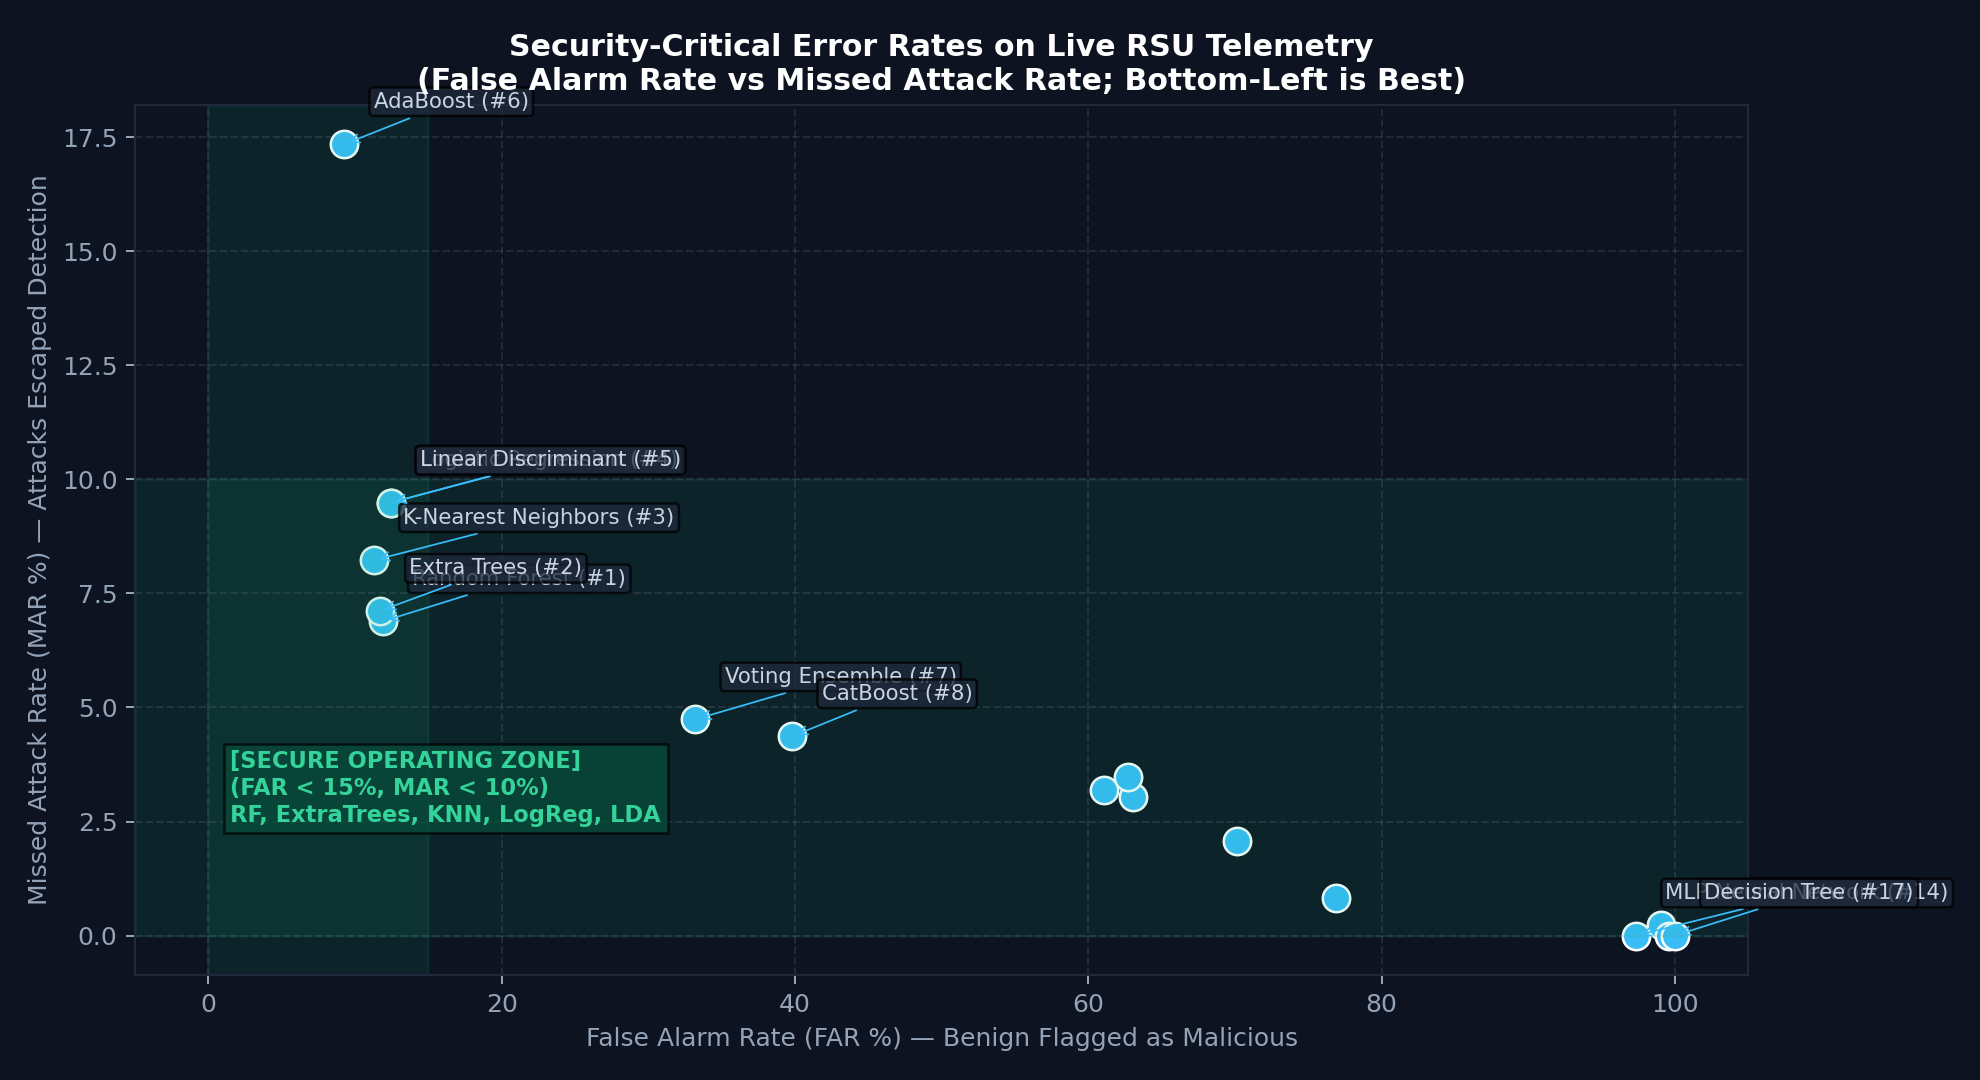
\includegraphics[width=\linewidth,keepaspectratio]{live_rsu_error_tradeoff.png}
        \column{0.38\textwidth}
        \footnotesize
        \begin{itemize}
            \item \textbf{Safety vs. Availability:}
            \begin{itemize}
                \item \textbf{Secure Operating Zone:} Random Forest, ExtraTrees, KNN, LogReg, and LDA achieve both False Alarm Rate $<15\%$ and Missed Attack Rate $<10\%$.
                \item \textbf{Radio Jitter Sensitivity:} Unregularized Decision Trees, SVM, and MLP suffer from $>97\%$ False Alarms under raw RF fading, proving deep neural nets are unsuited without spatial trust filtering.
            \end{itemize}
        \end{itemize}
    \end{columns}
\end{frame}

% =====================================================
% ADDITIONAL SLIDE: ADABOOST EDGE ANALYSIS (OPTIONAL)
% =====================================================
\begin{frame}{Edge Model Benchmark: AdaBoost vs. Remaining Classifiers}
    \framesubtitle{Rubric: Hardware Feasibility \& Lightweight Edge Inference}
    \centering
    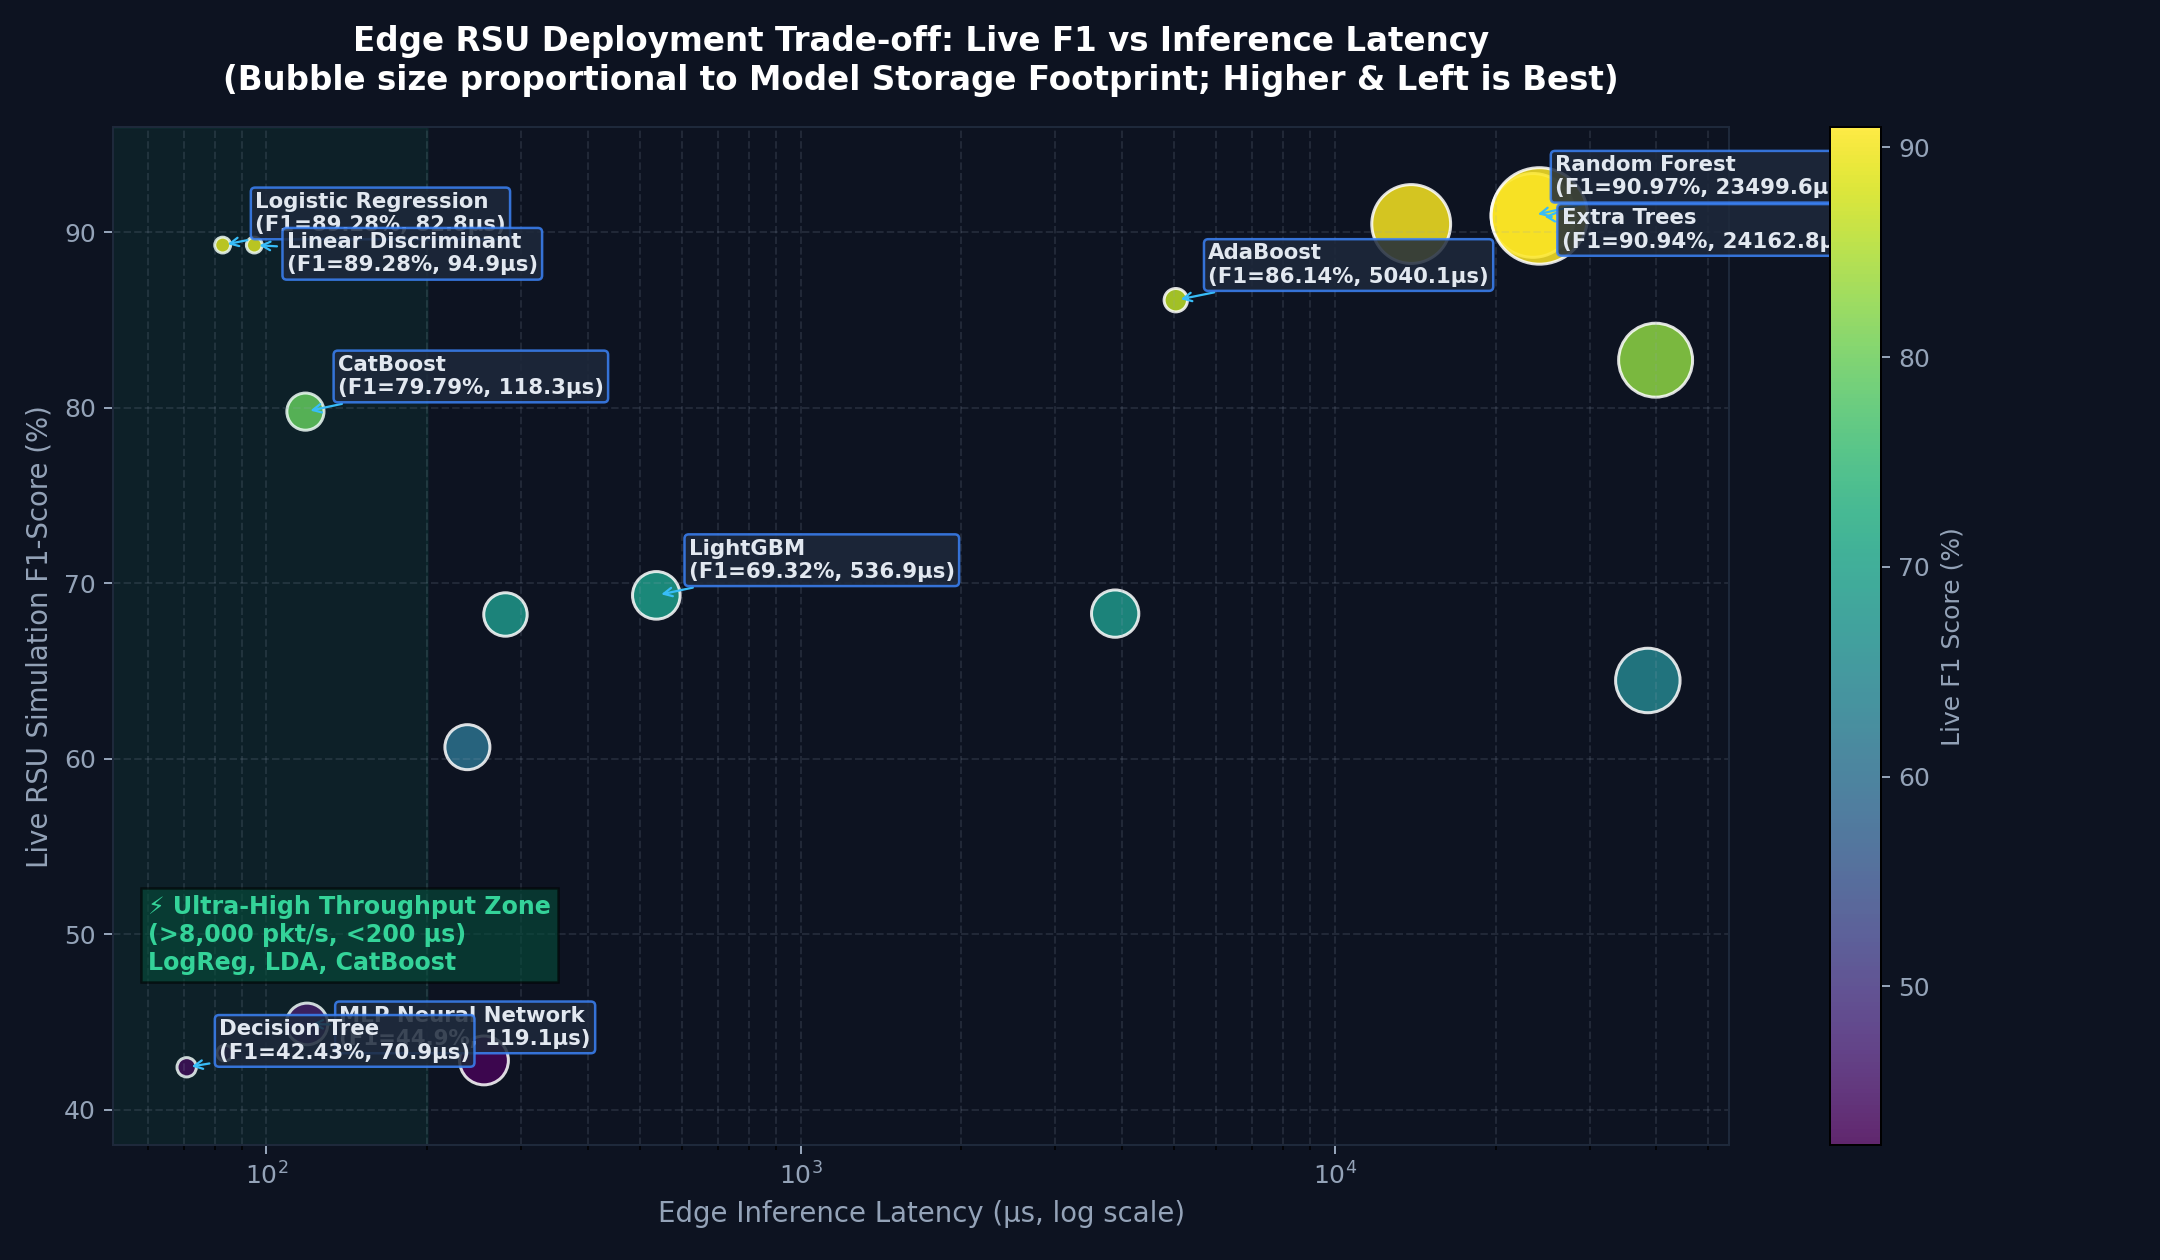
\includegraphics[width=\textwidth,height=0.82\textheight,keepaspectratio]{adaboost_edge_analysis.png}
\end{frame}

% =====================================================
% SLIDE: TECHNICAL KNOWLEDGE & DESIGN DECISIONS
% =====================================================
\section{Technical Knowledge}
\begin{frame}{10. Technical Knowledge \& Design Decisions}
    \framesubtitle{Rubric: Understanding of Methodology, Implementation \& Design Choices}
    \small
    \begin{itemize}
        \item \textbf{Why Tree Ensembles Win in Live Testing:} Vehicular telemetry exhibits sharp non-linear boundaries. Random Forest aggregates 150 orthogonal trees, filtering non-Gaussian radio noise to achieve the lowest missed attack rate (\textbf{6.89\%}) on 2{,}331 OMNeT++ live packets.
        \item \textbf{Eliminating Trajectory Leakage:} Enforced \textbf{GroupKFold by Vehicle ID (\texttt{node\_id})} (70/15/15) to prevent temporal autocorrelation leakage between train, validation, and test.
        \item \textbf{Why $\alpha = 0.70$ in EMA Trust Update:} Retains sufficient temporal memory to absorb transient radio fading while decisively dropping trust below 0.40 by packet 4 during attacks.
        \item \textbf{Two-Tier RSU Hybrid Architecture:} Tier 1 heuristic trust filter runs in $O(1)$ on all BSMs; Tier 2 ML model predicts misbehavior. Requires \textbf{both} low trust ($< 0.40$) \textbf{and} ML malicious prediction to \textbf{BLOCK}, ensuring zero false disconnects.
        \item \textbf{Validation vs. Live Testing Protocol:} Validated on 3{,}539 split dataset samples (\textbf{97.74\% F1}, CV: $96.95\% \pm 1.12\%$); independently tested on 2{,}331 live OMNeT++/Veins RSU packets (\textbf{90.99\% Acc}).
    \end{itemize}
\end{frame}
